%\documentclass[dvips]{beamer}
%\documentclass[10pt,xcolor=dvipsnames,mathserif]{beamer} % use option handout for handout
\documentclass{beamer}[11pt]
%\documentclass[handout]{beamer} %Pausen werden nicht berücksichtigt
%\documentclass[dvips,notes=onlyslideswithnotes]{beamer}
%\documentclass[pdftex]{beamer} %kompiliert jpeg, ABER LaTex to PDF

\usepackage[utf8]{inputenc}

\usepackage[scaled=1]{helvet}    %% --- Helvetica (Arial)
%\usepackage{courier}
%\usepackage[pdftex]{graphicx}
%\usepackage{textcomp}
\usepackage{epstopdf}
\usepackage{natbib,amssymb,rotating,subfigure}
\usepackage{amsmath}
\usepackage{amsthm}
\usepackage{amsfonts}
\usepackage{amssymb}
%\usepackage{breqn}			%Use the dmath-environment to break math eq. automatically!
\usepackage{makeidx}
\usepackage{txfonts}
\usepackage{colortbl}
\usepackage{moreverb}
\usepackage{eurosym}
\usepackage{verbatim}
%\hypersetup{colorlinks,linkcolor=blue,urlcolor=links}
\usepackage[ngerman]{babel}
\usepackage{color}
\usepackage{dcolumn,booktabs}
\usepackage{graphicx}
\usepackage{caption}
%\usepackage{llncs}
\usepackage{supertabular}
%\usepackage{threeparttable}
\usepackage[flushleft]{threeparttable}


\newcommand{\subsize}[1]{\tiny{#1}}

% Tables
\usepackage{booktabs}
\usepackage{multirow}


%Templates
% 1
%\mode<presentation>
%{
%  \usetheme{default} % Singapore % Montpellier
%  \setbeamercovered{transparent}
%	\setbeamertemplate{footline}[page number]
%	\setbeamertemplate{navigation symbols}{}
%}
\mode<presentation>
{
	\usetheme{CambridgeUS}%{default} % Singapore % Montpellier
	\setbeamercovered{transparent}
	%\setbeamertemplate{footline}[page number]
	%\setbeamertemplate{navigation symbols}{}
	\useinnertheme{rectangles}
}

%\pgfdeclareimage[height=1cm]{logo}{ecbLogo}
%\logo{\pgfuseimage{logo}}
%\usecolortheme{beaverJ}


% 2
\setbeamertemplate{sections/subsections in toc}[square]
\setbeamertemplate{navigation symbols}{} % suppresses all navigation symbols:

% %\usetheme{Madrid}
%\usetheme{Singapore}
% %\usecolortheme[named=NavyBlue]{structure}
%\useinnertheme{rectangles}


%%%%%%%%%%%
\def\newblock{\hskip .11em plus .33em minus .07em}
\newcolumntype{d}[1]{D{.}{.}{#1}}



\definecolor{myRed}{rgb}{0.8,0,0}
\definecolor{jirkasblue}{rgb}{0.2,0.2,0.7}
\definecolor{jirkasred}{rgb}{0.9,0,0}
%\newcommand{\jemph}[1]{{\color{jirkasred}#1}}
\newcommand{\remph}[1]{{\color{myRed}#1}}
\newcommand{\rbsymbol}[1]{\jemph{\boldsymbol{#1}}}   % "rb" stands for redbold
\definecolor{myGray}{rgb}{0.2,0.2,0.2}
\definecolor{jirkasgray}{rgb}{0.8,0.8,0.8}
\newcommand{\jemph}[1]{{\color{jirkasgray}#1}}
%\newcommand{\remph}[1]{{\color{myGray}#1}}
\newcommand{\gbsymbol}[1]{\jemph{\boldsymbol{#1}}}   % "gb" stands for redbold


\title{\textsc{Gretl und Hansl}}
\subtitle{Statistik und Ökonometrie anwenden mit freier Software}

\author[Tarassow] % (optional, for multiple authors)
{Artur Tarassow\inst{1}\\
	\textsc{\small }
	}

\institute[] % (optional)
{
  \inst{1}%
  Fachbereich Wirtschaft\\
  Technische Hochschule
}

\date[] % (optional)
{Brandenburg an der Havel, 17.01.2024}

%***********************************************************************************************
\begin{document}

\begin{frame}
	\titlepage
\end{frame}


\begin{frame}
	\frametitle{Outline}
	\tableofcontents%[pausesections]
\end{frame}


\section{Zweck und allgemeiner Charakter}


\begin{frame}{Zweck und allgemeiner Charakter}
	Hauptzwecke der Ökonometrie und Statistik:\footnote{Der folgende Inhalt basiert auf früheren Folien von von Allin Cottrell (Wake Forest University) and Riccardo "Jack" Lucchetti (Università Politecnica delle Marche).}

	\begin{itemize}
		\item Testen von Theorien
		\item Prognostik
		\item Politikevaluation
	\end{itemize}

	\medskip

	\emph{Anwendung} ökonomischer und statistischer Theorien auf Basis sozio-ökonomischer Daten.

	\medskip

	Aber auch \emph{Entwicklung} statistischer Theorien.
\end{frame}


\begin{frame}{Doppelter Status der Ökonometrie}
	Die Ökonometrie ist nicht ein "Teilgebiet" der Wirtschaftswissenschaften im gleichen Sinne wie z. B. Arbeitsökonomie oder Gesundheitsökonomie.

	\medskip

	Vielmehr ein Set von \emph{Werkzeugen}, die in fast allen Teilgebieten eingesetzt werden (außer in der reinen Theorie) -- plus ein Fachgebiet, das ebenso viel mathematische Statistik wie Wirtschaftswissenschaften ist.

	\medskip

	Jedoch ist ein Ökonometriker auch kein Statistiker: ein Ökonometriker ist ein Wirtschaftswissenschaftler mit einem überdurchschnittlichen Verständnis von Statistik.
\end{frame}


\section{Ökonometriesoftware}

\begin{frame}{Ökonometrie-Codierung}
	\begin{itemize}
		\item Pioniere der 1960er Jahre verwendeten hauptsächlich Fortran (einige große Namen verwenden dies noch)
		\item In der frühen PC-Ära gab es Kommandozeilenprogramme, die vorgefertigte Routinen anboten
		\item Gauss (1984, MS-DOS), Matlab (ebenfalls 1984), Ox (gegen 1997)
		\item 1990er bis heute: Entwicklung von Kommandozeilenprogrammen: Hinzufügen von GUIs und auch Elemente matrixorientierter Sprachen (Stata, 1985; Eviews, 1994)
		\item Jüngste Tendenz: Pakete, die auf matrixorientierten Sprachen aufbauen (Dynare)
		\item Auch: Weg von domänen-spezifischen Sprachen hin zu allgemeinen Sprachen (Python, Julia)
	\end{itemize}
\end{frame}


\begin{frame}{Numerische Verfahren in der Ökonometrie}
	\begin{itemize}
		\item Weit verbreitete Verwendung von Matrizen (hauptsächlich reell, nur selten komplex)
		\item Klassische Optimierungstechniken für stetige Funktionen %(schickere Sachen wie Genalgorithmen werden auch verwendet, aber sparsam)
		\item Zufallszahlengenerator (RNG) (zunehmend beliebt, insbesondere für bayesianische Verfahren)
		\item Einige Konzepte aus der Ingenieurliteratur: Spektren, Filterung, Signalextraktion.
	\end{itemize}
	\medskip

	Traditionell ist die Dimensionalität von Problemen relativ klein: Ein paar KB RAM reichen oft aus, um Daten zu speichern. Dies ändert sich heutzutage mit 'Big Data'-Problemen rapid.
\end{frame}



\begin{frame}{Der 'Markt' bzw. Anwendungen für ökonometrische Software}
	\begin{enumerate}
		\item Bachelor- und Masterstudiengänge (eine große Branche)
		\item Professionelle angewandte Arbeit
		      \begin{enumerate}
			      \item akademische Nutzung (hauptsächlich Universitäten)
			      \item geschäftliche Nutzung (traditionell große Finanzinstitute, aber heutzutage auch große Einzelhändler wie Amazon/ Google)
			      \item Politik (Zentralbanken, andere Regierungs-/supranationale Institutionen)
		      \end{enumerate}
		\item Entwicklung neuer Schätzer/ Werkzeuge
	\end{enumerate}

	Derzeit von proprietärer Software dominiert -- wie z.B. Stata und Eviews (für 1 und 2), plus Matlab und Python (für 2.3 und 3).
	\medskip

	Aber auch Verbreitung von R und Gretl, und geringe Verwendung von lower-level Programmiersprachen für Verwendung 3.
	\medskip

	Sehr wenige Menschen benutzen kompilierte Sprachen (C, Fortran usw.); selbst nicht für rechenintensive Aufgaben.
\end{frame}


\section{Einige Hintergrundinformationen zu Gretl}

\begin{frame}{Einige Hintergrundinformationen zu Gretl \textbf{I}}
	\begin{itemize}
		\item Akronym für:
		      \textbf{G}nu \textbf{R}egression, \textbf{E}conometrics und \textbf{T}ime-series \textbf{L}ibrary
		\item URL: \url{http://gretl.sourceforge.net/}
		\item Besteht aus
		      \begin{enumerate}
			      \item einer großen Shared Library (lib-gretl)
			      \item einem gemeinsamen Kommandozeilenprogramm (gretlcli)
			      \item und einem GUI-Client (gretl)
		      \end{enumerate}
		\item Verwendung zuverlässiger open-source Pakete, z.B. (multithreaded) LAPACK/BLAS, fftw, GTK, gnuplot, etc.
	\end{itemize}
\end{frame}


\begin{frame}{Einige Hintergrundinformationen zu Gretl \textbf{II}}
	\begin{itemize}
		\item Erste Version wurde im Januar 2000 veröffentlicht
		\item Wird seitdem aktiv weiterentwickelt $\to$ \textit{Open-Source} und \textit{kostenlos}.
		\item In C geschrieben und für Windows, OS X und Linux verfügbar.
		\item Benutzeroberfläche ist in 16 Sprachen verfügbar.
		\item Gretl ist in einem \textit{Benutzerhandbuch} von über 467 Seiten und einem \textit{Kommandoreferenz} von über 267 Seiten dokumentiert
	\end{itemize}
\end{frame}


\begin{frame}{Einige Hintergrundinformationen zu Gretl \textbf{III}}
	\begin{itemize}
		\item Gretl verfügt über eine voll ausgestattete grafische Benutzeroberfläche (GUI).
		\item Ausführung von Befehlen und Funktionen via Hansl-Skripting oder durch die GUI gesteuert.
	\end{itemize}

	\vspace{0.5cm}
	\textbf{Alleinstellungsmerkmal}

	\begin{itemize}
		\item Gretl bietet eine \textbf{hoch entwickelte matrix-orientierte Sprache} ähnlich zu Matlab und Gauss
		\item \textbf{UND} eine hoch entwickelte Sprache, die auf \textbf{Ökonometrie/ Statistik} abgestimmt ist.
	\end{itemize}
\end{frame}


\section{Datensätze und Matrizen}

\begin{frame}{Datensätze}
	Ein Datensatz ist im Wesentlichen die Vereinigung der Matrizen $\textbf{y}$ (T x k) und $\textbf{X}$ (T x m) mit zusätzlichen Metadaten.
	\begin{itemize}
		\item Drei Datentypen sind relevant: (i) Querschnitt, (ii) Zeitreihe und (iii) Panel.
		\item Betrachten Sie einen Datensatz als eine große Matrix. Um eine Regression zu verstehen, muss man wissen:
		      \begin{itemize}
			      \item Worauf beziehen sich die Spalten und Zeilen?
			      \item Repräsentation der Reihen als Zeitperioden: (i) Beginn und Ende der Stichprobe, (ii) Frequenz, mit der Daten erfasst wurden?
		      \end{itemize}
		\item In ökonometrischer Software ist der Datensatz typischerweise nicht als solche eine Matrix, sondern eine reichhaltigere Struktur und umfasst Metadaten. %%\\
		      %$ \Rightarrow $ ein Teil oder der gesamte Datensatz kann auf Anfrage in eine Matrix umgewandelt werden.
	\end{itemize}
\end{frame}


\begin{frame}{Datensätze}
	\textbf{1. Dualität} in Hansl: die Verfügbarkeit des \textit{Datensatzes} als einer spezifischen Datenstruktur neben Computerdarstellungen des Standardmathematischen Typs.

	\begin{itemize}
		\item Datensatz (plus Serien, Listen von Serien)
		\item \textit{Bundle} (als Träger-Objekt für weitere Datentypen; eine Art \textit{dictionary})
	\end{itemize}

	\textbf{2. Dualität}
	\begin{itemize}
		\item Matrizen, Skalare, Zeichenfolgen, Arrays, Bündel, Funktionen (schwieriger aber flexibler) \emph{versus}
		\item Datensätze, Serien, Befehle (einfach)
	\end{itemize}

	\vspace{0.5cm}

	Abschwächung der Dualität durch \underline{Zugriffselemente}, die nach Befehlen verwendet werden können. %(Nicht-triviale Befehle werden etwas funktionsähnlich.)
\end{frame}


\section{Datentypen}

\begin{frame}[fragile]{Skalare oder Matrizen}
	\begin{columns}[T] % align columns
		\begin{column}{.5\textwidth}
			\textbf{Kommando}
			\begin{verbatim}
				scalar a = 1.5
				scalar b = -2

				print a b

				matrix m = { 1, 2, 3;\
							             4, 5, 6 }

				matrix n = seq(1, 10, 2)

				print m n
			\end{verbatim}
		\end{column}

		\begin{column}{.5\textwidth}
			\textbf{Output}
			\begin{verbatim}
				a =  1.5000000

				b = -2.0000000

				m (2 x 3)
				1   2   3
				4   5   6

				n (1 x 5)
				1   3   5   7   9
			\end{verbatim}
	  \end{column}
	\end{columns}
\end{frame}

\begin{frame}[fragile]{Serien und Listen}
	\begin{columns}[T] % align columns
		\begin{column}{.5\textwidth}
			\textbf{Kommando}
			\begin{verbatim}
				# Erstelle Datensatz n=3
				nulldata 3

				# Zufalls-Variablen
				series y = normal()
				series x = normal()

				print y x -o

				list L = y x

				print L -o --range=1:2
			\end{verbatim}
		\end{column}

		\begin{column}{.5\textwidth}
			\textbf{Output}
			\begin{verbatim}
        				y            x

				1     0.373209    -1.846103
				2    -0.338461     1.076625
				3     1.053826    -1.874034

		         		y            x

				 1     0.373209    -1.846103
				 2    -0.338461     1.076625
			\end{verbatim}
	  \end{column}
	\end{columns}
\end{frame}


\begin{frame}[fragile]{Strings}
	\begin{columns}[T] % align columns
		\begin{column}{.5\textwidth}
			\textbf{Kommando}
			\begin{verbatim}
				set verbose off
				string s = "Hello world!"
				print s

				string a = "Hier ist"
				string b = " Gretl!"
				string c = a ~ b

				print c
			\end{verbatim}
		\end{column}

		\begin{column}{.5\textwidth}
			\textbf{Output}
			\begin{verbatim}
				Hello world!
				Hier ist Gretl!
			\end{verbatim}
	  \end{column}
	\end{columns}
\end{frame}


\begin{frame}[fragile]{Arrays -- Strings}
	\begin{columns}[T] % align columns
		\begin{column}{.5\textwidth}
			\textbf{Kommando}
			\begin{verbatim}
				set verbose off
				strings S = array(2)
				S[1] = "Hello"
				S[2] = "world!"
				print s

				S += "Hier
				print S
			\end{verbatim}
		\end{column}

		\begin{column}{.5\textwidth}
			\textbf{Output}
			\begin{verbatim}
				Hello world!
				Array of strings, length 3
				[1] "Hello"
				[2] "world!"
				[3] "Hier ist Hier ist "

				Array of strings, length 2
				[1] "world!"
				[2] "Hier ist Hier ist "
			\end{verbatim}
	  \end{column}
	\end{columns}
\end{frame}

\begin{frame}[fragile]{Arrays -- Matrizen}
	\begin{columns}[T] % align columns
		\begin{column}{.5\textwidth}
			\textbf{Kommando}
			\begin{verbatim}
				set verbose off
				matrices M = array(2)
				M[1] = { 1, 2, 3;\
							         4, 5, 6 }

				M[2] = seq(1, 10, 2)

				print M

				print M[1]
				print M[2]
			\end{verbatim}
		\end{column}

		\begin{column}{.5\textwidth}
			\textbf{Output}
			\begin{verbatim}



				Array of matrices, length 2
				[1] 2 x 3
				[2] 1 x 5

				1   2   3
				4   5   6

				1   3   5   7   9
			\end{verbatim}
	  \end{column}
	\end{columns}
\end{frame}


\begin{frame}[fragile]{Bundle}
	\small
	\begin{columns}[T] % align columns
		\begin{column}{.55\textwidth}
			\textbf{Kommando}
			\begin{verbatim}
				set verbose off

				bundle B = _(a = "Hello, world!",
							 b = -1.5,
							 c = { 1, 2, 3; 4, 5, 6 },
							 d = defarray("A", "B", "C"))

				print B

				print B.a
				print B["d"]

				B.b = 33
				print B.b
			\end{verbatim}
		\end{column}

		\begin{column}{.45\textwidth}
			\textbf{Output}
			\begin{verbatim}
				bundle B:
				b = -1.5
				c (matrix: 2 x 3)
				a = "Hello, world!"
				d = array of strings, length 3

				Hello, world!
				Array of strings, length 3
				[1] "A"
				[2] "B"
				[3] "C"

				33
			\end{verbatim}
	  \end{column}
	\end{columns}
\end{frame}


\section{Skriptsprache Hansl}


\begin{frame}{Hansl -- Hansl's A Neat Scripting Language}
	\begin{itemize}
		\item Der Werdegang der Gretl-Entwicklung ist der proprietärer Software ähnlich (DOS-Kommandozeilenprogramm $\to$ Cross-Plattform $\to$ GUI hinzufügen $\to$ Matlab-ähnliche Matrixfunktionalität hinzufügen $\to$ Erweitertes Scripting hinzufügen $ \to $ Parallelisierung) %\pause
		\item 'Gefühl' der Skriptsprache hat Ähnlichkeiten zur Bash Shell (UNIX).
		\item C-Back-End (natürlich mit ein wenig Hilfe von Freunden: netlib, BLAS, lapack, FFTW und anderen)
		\item Übergang zur Entwicklung von Gretl über Hansl (Funktionspakete mit optionaler GUI-Integration)
		\item Einige 'Legacy'-Formulierungen und Inkonsistenzen, aber Hansl ist sauber und einfach zu lernen
	\end{itemize}
\end{frame}


\begin{frame}{Hansl -- Befehle}
	Hansl umfasst mehr 204 Befehle:\footnote{\url{https://gretl.sourceforge.net/gretl-help/cmdref.html}}
	\begin{itemize}
		\item Tests (Hypothese)
		\item Statistik und Wahrscheinlichkeitsrechnung
		\item Datensatz (Manipulation, Sortierung, usw.)
		\item Schätzung (OLS, MLE, GMM, Einzelgleichung und Systeme usw.)
		\item Graphen (Streudiagramme, Boxplots, Zeitreihen, usw.)
		\item Programmierung (Steuerungsfluss und Fehlersuche)
		\item Transformationen
		\item String-Operationen
		\item Prognostik
	\end{itemize}
\end{frame}


\begin{frame}{Hansl -- Funktionen}
	Hansl umfasst etwa 250 Funktionen:\footnote{\url{https://gretl.sourceforge.net/gretl-help/funcref.html}}
	\begin{columns}[T] % align columns
		\begin{column}{.5\textwidth}
			\begin{itemize}
				\item mathematische
				\item statistische
				\item Strings
				\item Daten-Tools
				\item Programmierung
				\item numerische Methoden
			\end{itemize}
		\end{column}

		\begin{column}{.5\textwidth}
			\begin{itemize}
				\item Matrix-Manipulation
				\item Zeitreihen
				\item Transformationen
				\item Komplexe Zahlen
				\item Wahrscheinlichkeitsrechnung
				\item Lineare Algebra
				\item Kalenderfunktionen
				\item nicht-parametrische Modelle
			\end{itemize}
	  \end{column}
	\end{columns}
\end{frame}

\section{Modelle und Methoden}

\begin{frame}{Modelle}
	Implementiert sind eine Vielzahl von Modellen und Methoden
	\begin{itemize}
		\item Zeitreihenmethoden
		      \begin{itemize}
			      \item ARIMA, univariate GARCH-Typ, (S)VARs und VECMs, Einheitswurzel- und Gleichgewichtstests, Kalman-Filter, MIDAS, Echtzeit-Datensätze
		      \end{itemize}
		\item Begrenzt abhängige Variablen
		      \begin{itemize}
			      \item logit, probit, tobit, Stichprobenselektion, Intervallregulierung, Modelle für Zähler- und Dauerdaten usw.
		      \end{itemize}
		\item Panelldatenschätzer, einschließlich Instrumentvariablen, Probit- und GMM-basierter dynamischer Panelmodelle
		\item Maschinelles Lernen: Ridge, LASSO, Elastic-Net, SVM, Random Forests (via R)
	\end{itemize}
\end{frame}


\begin{frame}{3rd-party Pakete von Nutzern}
	Derzeit werden über 100 nutzergeschriebene Pakete bereitgestellt.
	\medskip

	Siehe hier:
	\medskip

	\url{https://gretl.sourceforge.net/cgi-bin/gretldata.cgi?opt=SHOW_FUNCS}
\end{frame}


\begin{frame}[fragile]{Installieren und Laden von 3rd-party Paketen}
	\begin{verbatim}
		set verbose off
		# Installiere Paket vom Server
		pkg install PairPlot

		# Lade Paket in den Speicher
		include PairPlot.gfn

		# Zeige die Hilfe
		help PairPlot
	\end{verbatim}

	Beispiel-Skripte sind in jedem Gretl-Paket enthalten.
\end{frame}


\section{Dateiformate}

\begin{frame}{Unterstützte Datenformate}
	Unterstützte Formate, um Daten zu laden umfassen:

	\begin{itemize}
		\item Eigene XML-Datendatei (\texttt{*.gdt} und \texttt{*.gdtb})
		\item Komma-separierte Textdatei (txt, csv)
		\item Excel-Arbeitsblätter
		\item Gnumeric und OpenDocument-Arbeitsblätter
		\item Stata-Dateien (.dta)
		\item SPSS-Dateien (.sav)
		\item Eviews-Arbeitsdateien
		\item JMulTi-Datendateien
		\item Eigene Binärdatenbanken im eigenen Format (ermöglicht gemischte Datenfrequenzen und Serienlängen)
		\item RATS 4-Datenbanken und PC-Give-Datenbanken
		\item Beinhaltet eine Beispieldatenbank für die US-Wirtschaft. Weitere Informationen finden Sie auf der Gretl-Datenseite.
	\end{itemize}
\end{frame}


\begin{frame}{Kommunikation mit anderen Programmen}
	Gretl kann mit anderen Softwarepaketen interagieren.
	\medskip

	Datensätze und Matrizen einfach senden und empfangen.
	\medskip

	Andere Programme über Gretls \texttt{foreign-language}-Block aufrufen.
	\medskip

	Liste der unterstützten Software:

	\begin{itemize}
		\item R (noch mehr Unterstützung)
		\item Ox
		\item Octave
		\item Stata
		\item Python
		\item Julia
	\end{itemize}
\end{frame}


\begin{frame}[fragile]%{Gretl und R Beispiel}
	\textbf{Gretl und R Beispiel}
	\footnotesize
	\begin{verbatim}
	function list RStructTS(series myseries)
	  smpl ok(myseries) --restrict
	  sx = argname(myseries)
	  foreign language=R --send-data --quiet
	    @sx <- gretldata[, "myseries"]
	    strmod <- StructTS(@sx)
	    compon <- as.ts(tsSmooth(strmod))
	    gretl.export(compon)
	  end foreign
	  append @dotdir/compon.csv
	  rename level @sx_level
	  rename slope @sx_slope
	  rename sea @sx_seas
	  list ret = @sx_level @sx_slope @sx_seas
	  return ret
	end function
	# ------------ main -------------------------
	open bjg.gdt
	list X = RStructTS(lg)
	\end{verbatim}
\end{frame}


\begin{frame}{Materialien zu Gretl \textbf{I}}
	\begin{itemize}
		\item \textit{Material-on-Gretl} \url{https://github.com/gretl-project/material-on-gretl}
		\item \textit{Wiki 1} \url{https://github.com/gretl-project/material-on-gretl/wiki}
		\item \textit{Wiki 2} \url{https://gretlwiki.econ.univpm.it/index.php/Main_Page}
		\item \textit{Gretl Command Reference} \url{https://gretl.sourceforge.net/gretl-help/cmdref.html}
		\item \textit{Gretl User's Guide}: \url{http://sourceforge.net/projects/gretl/files/manual/}
	\end{itemize}
\end{frame}

\begin{frame}{Materialien zu Gretl \textbf{II}}
	\begin{itemize}
		\item \textit{gretl-users E-Mail-Liste}: Die meisten gut überlegten Fragen werden relativ schnell beantwortet und ausführlich beantwortet.
		   \url{https://gretlml.univpm.it/postorius/lists/gretl-users.gretlml.univpm.it/}
		\item Lehrbuch \textit{Using gretl for Principles of Econometrics} (5. Auflage) \url{http://www.learneconometrics.com/gretl/}
		\item Gretl Cheat-sheet \url{https://github.com/gretl-project/gretl_cheatsheet}
		\item \textit{Beispielskripts}: Das Gretl-Paket enthält eine Vielzahl von Beispiel- oder Übungsskripts (unter dem Menüpunkt /Datei/Skriptdateien/Übungsdatei).
		\item \textit{Funktionspakete}: Ambitionierte Beispiele für Hansl-Codierung (über den Gretl-Menüpunkt /Werkzeuge/Funktionspakete/Auf Server).)
	\end{itemize}
\end{frame}


\section{Mit dem Datensatz arbeiten}


\begin{frame}
	\centering
	\LARGE
	\textbf{Mit dem Datensatz arbeiten}
\end{frame}



\begin{frame}[fragile]{Serien erzeugen}
	\begin{columns}[T] % align columns
		\scriptsize
		\begin{column}{.4\textwidth}
			\begin{verbatim}
				set verbose off

				# Erstelle Datensatz n=3
				nulldata 3

				# Normalverteilte Zufallsvariable
				# mean = 4, std-dev = 0.5
				series y = normal(4, 0.5)

				series y_sq = y^2
				series log_y = log(y)
				series exp_y = exp(y)
				series x = {1, 2, 3}'

				series z = y - x

				print y y_sq log_y exp_y x z --byobs
			\end{verbatim}
		\end{column}

		\begin{column}{.6\textwidth}
			\tiny
			\begin{verbatim}
				             y         y_sq        log_y        exp_y        x
  				1     4.353309     18.95130     1.470936      77.7353     1
			   2     4.267813     18.21423     1.451102      71.3654     2
			   3     4.985425     24.85446     1.606519     146.2658     3

				          z

				   1     3.353309
				   2     2.267813
				   3     1.985425

			\end{verbatim}
	  \end{column}
	\end{columns}
\end{frame}


\begin{frame}[fragile]{Dummyvariablen erzeugen}
	\begin{columns}[T] % align columns
		\scriptsize
		\begin{column}{.62\textwidth}
			\begin{verbatim}
				open "./data/abdata.csv" --quiet --preserve

				# Dummyvariablen erzeugen
				series DUM = (YEAR == 1977 || YEAR == 1980)

				print YEAR DUM -o --range=1:10
			\end{verbatim}
		\end{column}

		\begin{column}{.4\textwidth}
			\tiny
			\begin{verbatim}
				gretl version 2024a-git
				Current session: 2024-01-16 13:35

				? print YEAR DUM -o --range=1:10

				            YEAR          DUM

				 1         1976            0
				 2         1977            1
				 3         1978            0
				 4         1979            0
				 5         1980            1
				 6         1981            0
				 7         1982            0
				 8         1983            0
				 9         1984            0
				10         1976            0
			\end{verbatim}
	  \end{column}
	\end{columns}
\end{frame}

\begin{frame}[fragile]{Metadaten für Serien hinzufügen}
	\begin{verbatim}
		nulldata 3
		series y = normal()

		# Beschreibung für Serie hinzufügen
		setinfo y --description="Some random number"

		# Anstelle von 'y' soll 'Cool variable'
		# bei Plots erscheinen
		setinfo y --graph-name="Cool variable"

		boxplot y --output=display
	\end{verbatim}
\end{frame}


\begin{frame}[fragile]{Werte ersetzen}
	\begin{columns}[T] % align columns
		\scriptsize
		\begin{column}{.55\textwidth}
			\begin{verbatim}
				set verbose off

				# Neuen Datensatz mit 4 Beobachtungen
				# erstellen
				nulldata 5 --preserve
				# Generiere Serie mit komischen Werten
				series weird_values = {5, 6, 10, 20, NA}'
				print weird_values --byobs

				# Let's replace values
				help replace
				matrix find = {5, 6, 10, 20, NA}
				matrix replace_by = {0, 1, 2, 3, -1}

				series y = replace(weird_values, find, replace_by)
				print weird_values y --byobs
			\end{verbatim}
		\end{column}

		\begin{column}{.45\textwidth}
			\tiny
			\begin{verbatim}
				weird_values

				1            5
				2            6
				3           10
				4           20
				5

				weird_values            y

				1            5            0
				2            6            1
				3           10            2
				4           20            3
				5                        -1
			\end{verbatim}
	  \end{column}
	\end{columns}
\end{frame}


\begin{frame}[fragile]{String-Werte in Series einfügen}
	\begin{columns}[T] % align columns
		\scriptsize
		\begin{column}{.6\textwidth}
			\begin{verbatim}
				set verbose off
				nulldata 20

				series y = randgen(i, 1, 3)
				setinfo y --description="3 different categories"

				print y --byobs --range=1:5

				# Create strings for categories 1, 2 and 3
				strings series_labels = defarray("Low income",\
				  "Medium income", "High income")
				# Attache strings to categorical series
				help stringify
				stringify(y, series_labels)

				print y --byobs --range=1:5
			\end{verbatim}
		\end{column}

		\begin{column}{.4\textwidth}
			\tiny
			\begin{verbatim}
				           y

				1            2
				2            3
				3            2
				4            1
				5            3


				        y

				1 Medium income
				2   High income
				3 Medium income
				4    Low income
				5   High income

			\end{verbatim}
	  \end{column}
	\end{columns}
\end{frame}




\section{Erste Schritte}


\begin{frame}[fragile]{Einlesen eines Datensatzes und Werte zeigen}
	\begin{columns}[T] % align columns
		\scriptsize
		\begin{column}{.45\textwidth}
			\begin{verbatim}
				clear
				set verbose off

				# Arbeitsordner definieren
				string DIR = "<PATH>"
				set workdir "@DIR"

				# Relative Pfadangabe zum
				# Ordner "data"
				open "./data/abdata.csv"

				# Zeige die ersten 10 Zeilen
				# einiger Serien
				list Y = IND YEAR n w k
				print Y --byobs --range=1:10
			\end{verbatim}
		\end{column}

		\begin{column}{.55\textwidth}
			\tiny
			\begin{verbatim}
			       IND      YEAR         n            w          k

				1                1976
				2      7         1977     1.617604     2.576543   -0.5286502
				3      7         1978     1.722767     2.509746   -0.4591824
				4      7         1979     1.612433     2.552526   -0.3899363
				5      7         1980     1.550749     2.624951   -0.4827242
				6      7         1981     1.409278     2.659539   -0.6780615
				7      7         1982     1.152469     2.699218   -0.8606196
				8      7         1983     1.077048     2.623102   -0.9364935
				9                1984
			10               1976
			\end{verbatim}
	  \end{column}
	\end{columns}
\end{frame}


\begin{frame}[fragile]{Datensatz um 'markers' (Beobachtungslabels) erweitern}
	\begin{columns}[T] % align columns
		\scriptsize
		\begin{column}{.55\textwidth}
			\begin{verbatim}
				nulldata 4
				series y = {1, 2, 3, 4}
				series x = normal()

				strings S = defarray("Artur", "Fritzi",
				  "Katharina", "Olga")
				markers --from-array=S

				print y x -o

				# Berühre die Datenunkte
				# und die Labels erscheinen
				gnuplot y x --output=display
			\end{verbatim}
		\end{column}

		\begin{column}{.45\textwidth}
			\scriptsize
			\begin{verbatim}
				            y            x

				Artur       1   -0.6772452
			Fritzi      2    0.4454971
			Katharina   3    0.4316438
				 Olga       4    0.1343885
			\end{verbatim}
	  \end{column}
	\end{columns}
\end{frame}


\begin{frame}[fragile]{Deskriptive Statistiken}
	\begin{columns}[T] % align columns
		\scriptsize
		\begin{column}{.45\textwidth}
			\begin{verbatim}
				list Y = IND YEAR n w k

				summary Y --simple



				# Statistiken je Jahr
				# wobei die Jahre
				# eingeschränkt werden
				list Y = n w k

				smpl YEAR >= 1976 \
				  && YEAR <= 1977 --restrict

				summary Y --by=YEAR --simple
			\end{verbatim}
		\end{column}

		\begin{column}{.55\textwidth}
			\tiny
			\begin{verbatim}
		         Mean      Median     S.D.      Min      Max
		IND      5.123      5.000     2.678    1.000    9.000
		YEAR      1980       1980     2.583     1976     1984
		n        1.056     0.8272     1.342   -2.263    4.687
		w        3.143      3.178    0.2630    2.082    3.812
		k      -0.4416    -0.6578     1.514   -4.431    3.852


		YEAR = 1976 (n = 80):

			              Mean     Median     S.D.      Min        Max
		n            1.239    1.033    1.382     -1.444      4.588
		w            3.237    3.266   0.2683      2.178      3.812
		k          -0.2912  -0.5390    1.518     -2.966      3.531

		YEAR = 1977 (n = 138):

			             Mean   Median    S.D.     Min     Max
		n            1.160   0.9683   1.340  -1.952   4.597
		w            3.129    3.169  0.2714   2.123   3.730
		k          -0.3876  -0.6218   1.472  -3.393   3.477
			\end{verbatim}
	  \end{column}
	\end{columns}
\end{frame}



\begin{frame}[fragile]{Aggregation}
	\begin{columns}[T] % align columns
		\scriptsize
		\begin{column}{.62\textwidth}
			\begin{verbatim}
				# Aggregiere die folgenden Variablen
				list Y = n w

				# Gruppiere nach der Variable IND
				list groupby = IND

				# Berechne den Mittelwert für 'Y' für jede
				# Ausprägung von 'groupby'
				matrix mean_values = aggregate(Y, groupby, "mean")

				# Optionale Formatierung des Outputs
				printf "\n%12.2f\n", mean_values
			\end{verbatim}
		\end{column}

		\begin{column}{.4\textwidth}
			\tiny
			\begin{verbatim}
				IND       count           n           w
				1.00       41.00        1.27        3.11
				2.00       32.00        1.23        3.50
				3.00       34.00        0.72        3.25
				4.00       76.00        1.44        3.32
			\end{verbatim}
	  \end{column}
	\end{columns}
\end{frame}


\begin{frame}[fragile]{Wegschreiben der Textausgabe}
	\begin{columns}[T] % align columns
		\small
		\begin{column}{.7\textwidth}
			\begin{verbatim}
				# Berechne den Mittelwert für 'Y' für jede
				# Ausprägung von 'groupby'
				matrix mean_values = aggregate(Y, groupby, "mean")

				# Textausgabe als txt-Datei speichern
				string filename = "./output/aggregation_mean_output.txt"

				outfile "@filename
					printf "\n%12.2f\n", mean_values
				end outfile
			\end{verbatim}
		\end{column}
	\end{columns}
\end{frame}


\begin{frame}[fragile]{Matrix als csv speichern und öffnen der csv}
	\begin{columns}[T] % align columns
		\small
		\begin{column}{.7\textwidth}
			\begin{verbatim}
				# Berechne den Mittelwert für 'Y' für jede
				# Ausprägung von 'groupby'
				matrix mean_values = aggregate(Y, groupby, "mean")

				# Speichern der Matrix als csv
				string filename = "./output/aggregation_als_matrix.csv"
				store "@filename" --matrix=mean_values

				# Matrix-csv als Datensatz einlesen für
				# weitere Bearbeitung
				open "@filename" --preserve
			\end{verbatim}
		\end{column}
	\end{columns}
\end{frame}


\begin{frame}[fragile]{Sample restringieren}
	\begin{columns}[T] % align columns
		\scriptsize
		\begin{column}{.62\textwidth}
			\begin{verbatim}
				open abdata --quiet

				list Y = IND YEAR n w

				# Statistiken für alle Beobachtungen
				summary Y --simple

				# Statistiken für Jahre zw. 1976 - 1978
				smpl YEAR >= 1976 && YEAR <= 1978 --restrict
				summary Y --simple

				# Wiederherstellen des vollen Datensatzes
				summary Y --simple
			\end{verbatim}
		\end{column}

		\begin{column}{.4\textwidth}
			\tiny
			\begin{verbatim}
				IND       count           n           w
				1.00       41.00        1.27        3.11
				2.00       32.00        1.23        3.50
				3.00       34.00        0.72        3.25
				4.00       76.00        1.44        3.32
			\end{verbatim}
	  \end{column}
	\end{columns}
\end{frame}



\begin{frame}[fragile]{KQ Regression}
	\begin{columns}[T] % align columns
		\scriptsize
		\begin{column}{.45\textwidth}
			\begin{verbatim}
				# Conduct OLS regression (optionally with robust standard errors)
				ols ys const n w  #--robust

				# Store coefficients
				matrix coeff = $coeff

				# Store standard errors
				matrix stderr = $stderr

				# Store residuals
				series uhat = $uhat

				# Store fitted values
				series yhat = $yhat

				# Store R^2
				scalar r2 = $rsq
			\end{verbatim}
		\end{column}

		\begin{column}{.55\textwidth}
			\tiny
			\begin{verbatim}



				Model 9: OLS, using observations 1-1260 (n = 1031)
				Missing or incomplete observations dropped: 229
				Dependent variable: ys

							 coefficient   std. error   t-ratio    p-value
				  --------------------------------------------------------
				  const      4.60388       0.0351033    131.2      0.0000  ***
				  n          0.00626942    0.00217539     2.882    0.0040  ***
				  w          0.00875566    0.0110959      0.7891   0.4302

				Mean dependent var   4.638015   S.D. dependent var   0.093961
				Sum squared resid    9.015800   S.E. of regression   0.093650
				R-squared            0.008551   Adjusted R-squared   0.006622
				F(2, 1028)           4.433125   P-value(F)           0.012105
				Log-likelihood       980.1866   Akaike criterion    -1954.373
				Schwarz criterion   -1939.558   Hannan-Quinn        -1948.751
			\end{verbatim}
	  \end{column}
	\end{columns}
\end{frame}


\begin{frame}[fragile]{Spezifikationstests}
	\begin{columns}[T] % align columns
		\scriptsize
		\begin{column}{.45\textwidth}
			\begin{verbatim}
				# See the help on tests
				help modtest

				# Conduct OLS regression
				ols ys const n w  #--robust

				# Tests are conducted for the
				# last model estimated

				# Normality test
				modtest --normality --quiet

				# White's test on homoscedasticity
				modtest --white
				scalar teststat_white = $test
				scalar pvalue_white = $pvalue

				# RESET test on functional form
				reset --squares-only
			\end{verbatim}
		\end{column}

		\begin{column}{.55\textwidth}
			\tiny
			\begin{verbatim}
				Test for null hypothesis of normal distribution:
				Chi-square(2) = 82.810 with p-value 0.00000


				White's test for heteroskedasticity
				Test statistic: TR^2 = 29.920521,
				with p-value = P(Chi-square(5) > 29.920521) = 0.000015


				RESET test for specification (squares only)
				Null hypothesis: specification is adequate
				Test statistic: F = 12.054076,
				with p-value = P(F(1,1027) > 12.0541) = 0.000538
			\end{verbatim}
	  \end{column}
	\end{columns}
\end{frame}


\begin{frame}[fragile]{Testen von Restriktionen}
	\begin{columns}[T] % align columns
		\scriptsize
		\begin{column}{.5\textwidth}
			\begin{verbatim}
				# Restriktionen
				ols ys const n w

				# t-Test: H0: beta(n) = 0,
				# H1: beta(n) != 0
				help omit
				omit n --test-only

				# F-Test: H0: beta(n) = beta_(w) 0,
				# H1: beta(n) != 0 und/ oder
				# beta_(w) != 0
				list drop = n w
				omit drop --test-only

				# More flexible: the restrict-block
				help restrict

				restrict # --bootstrap
			      b[const] = 4
				  b[w] = 0.1
				end restrict
			\end{verbatim}
		\end{column}

		\begin{column}{.53\textwidth}
			\tiny
			\begin{verbatim}
				Test on Model 13:
				Null hypothesis: the regression parameter is zero for n
				Test statistic: F(1, 1028) = 8.30579, p-value 0.00403412

				Test on Model 13:
				Null hypothesis: the regression parameters are
				zero for the variables
					n, w
				Test statistic: F(2, 1028) = 4.43312, p-value 0.0121052


				Restriction set
				1: b[const] = 4
				2: b[w] = 0.1

				Test statistic: F(2, 1028) = 3675.38, with p-value = 0
			\end{verbatim}
	  \end{column}
	\end{columns}
\end{frame}


\begin{frame}[fragile]{Zusammenfassung Regressionsergebnisse eines Modells}
	Speicher Regressionsergebnisse als RTF- (Word) oder tex-Datei.
	\begin{columns}[T] % align columns
		\scriptsize
		\begin{column}{.5\textwidth}
			\begin{verbatim}
				open "./data/abdata.csv" --quiet --preserve

				ols ys const n w --simple

				tabprint --output="./output/regression_output.rtf"
			\end{verbatim}
		\end{column}

		\begin{column}{.53\textwidth}
			\tiny
			\begin{verbatim}

			\end{verbatim}
	  \end{column}
	\end{columns}

	\vspace{0.5cm}
	Alternativ für tex-Dateien auch der Befehl \texttt{eqnprint}.
\end{frame}


\begin{frame}[fragile]{Zusammenfassung Regressionsergebnisse mehrer Modelle}
	Speicher Regressionsergebnisse mehrer Modelle als RTF- (Word) oder tex-Datei.

	\scriptsize
	\begin{verbatim}
		open abdata.gdt --quiet --preserve
		modeltab free
		m1 <- ols ys const --quiet
		modeltab add

		m2 <- ols ys const n --quiet
		modeltab add

		m3 <- ols ys const n w --quiet
		modeltab add

		modeltab show
		modeltab --output="./output/regression_table.rtf"
	\end{verbatim}
\end{frame}



\section{Plotting}

\begin{frame}
	\centering
	\LARGE
	\textbf{Daten plotten}
\end{frame}

\begin{frame}{Plotting}
	\begin{itemize}
	  \item Gnuplot als Plotting-Engine (sehr leistungsfähig) (\url{http://www.gnuplot.info/})
	  \item Es gibt für die grundlegenden Plots bereits native Unterstützung in Gretl
	  \item Hier einige Beispiel
	\end{itemize}
\end{frame}


\begin{frame}[fragile]{Scatterplot}
	\begin{columns}[T] % align columns
		\small
		\begin{column}{.4\textwidth}
			\begin{verbatim}
				set verbose off

				open mroz87.gdt

				gnuplot WE log(FAMINC) \
				  --output=display
			\end{verbatim}
		\end{column}

		\begin{column}{.6\textwidth}
			\begin{figure}
				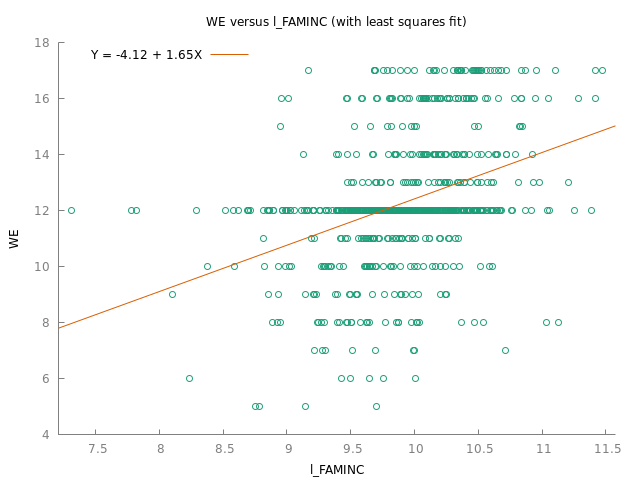
\includegraphics[width=1.0\textwidth]{../figures/scatterplot.png}
				\caption{Scatterplot mit Gretl}
			\end{figure}
	  \end{column}
	\end{columns}
\end{frame}


\begin{frame}[fragile]{Scatterplot mit markers}
	\begin{columns}[T] % align columns
		\small
		\begin{column}{.6\textwidth}
			\begin{verbatim}
				open mrw.gdt --quiet

				gnuplot gdp60 school --output=display
			\end{verbatim}
			\textbf{Recht-klick in den Plot und dann "All data labels" auswählen.}
		\end{column}

		\begin{column}{.4\textwidth}
			\begin{verbatim}
				                 school

				Algeria          4.5
				 Angola          1.8
				  Benin          1.8
			Botswana          2.9
				Burkina          0.4
			\end{verbatim}
	  \end{column}
	\end{columns}
\end{frame}


\begin{frame}[fragile]{Scatterplot mit Dummyausprägungen}
	\begin{columns}[T] % align columns
		\tiny
		\begin{column}{.4\textwidth}
			\begin{verbatim}
				set verbose off

				open mroz87.gdt

				gnuplot WE log(FAMINC) CIT --dummy \
				  --output="scatterplot_factorized.png" \
				  { set title "Some cool title" font ',15';\
				  set linetype 1 lc rgb 'orange' ps 1;\
				  set linetype 2 lc rgb 'blue' ps 0.5;\
				  set xtics font ',15';\
				  set grid;}
			\end{verbatim}
		\end{column}

		\begin{column}{.6\textwidth}
			\begin{figure}
				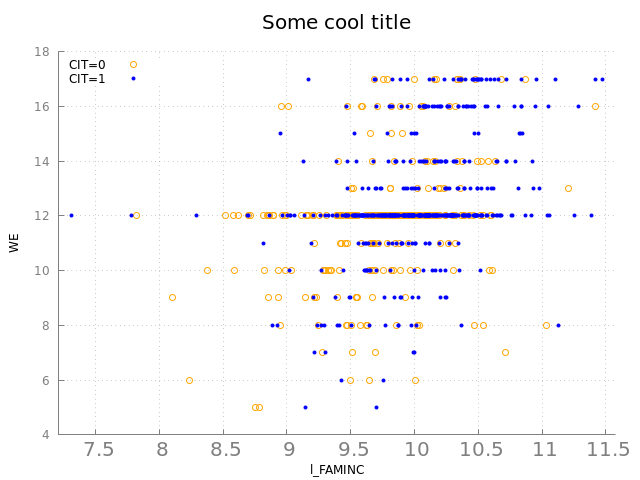
\includegraphics[width=1.0\textwidth]{../figures/scatterplot_factorized.png}
				\caption{Scatterplot mit separaten Punkten je Ausprägung der Dummy-Variable \texttt{CIT}}
			\end{figure}
	  \end{column}
	\end{columns}
\end{frame}

\begin{frame}[fragile]{Scatterplot-Matrix}
	\begin{columns}[T] % align columns
		\small
		\begin{column}{.42\textwidth}
			\begin{verbatim}
				set verbose off

				open mroz87.gdt

				list Y = WHRS WW HHRS

				scatters WE ; Y \
				  --output=display
			\end{verbatim}
		\end{column}

		\begin{column}{.6\textwidth}
			\begin{figure}
				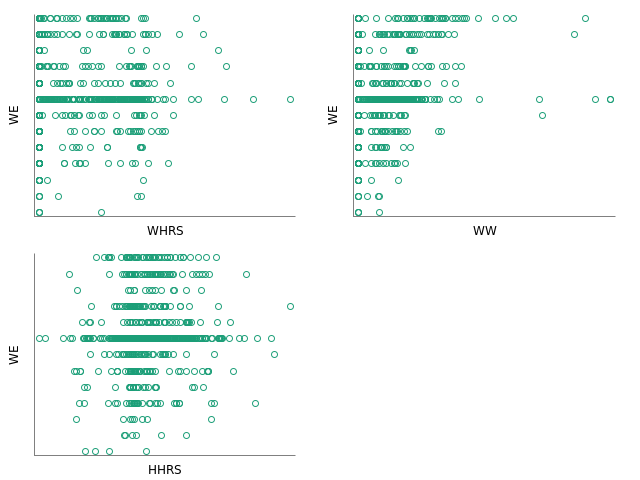
\includegraphics[width=1.0\textwidth]{../figures/scatters_matrix.png}
				\caption{Scatterplot mit \texttt{WE} auf der x-Achse aber verschiedenen Variablen auf der y-Achse}
			\end{figure}
	  \end{column}
	\end{columns}
\end{frame}


\begin{frame}[fragile]{Boxplot}
	\begin{columns}[T] % align columns
		\scriptsize
		\begin{column}{.4\textwidth}
			\begin{verbatim}
				set verbose off
				open mroz87.gdt

				boxplot FAMINC --output=display
			\end{verbatim}
		\end{column}

		\begin{column}{.6\textwidth}
			\begin{figure}
				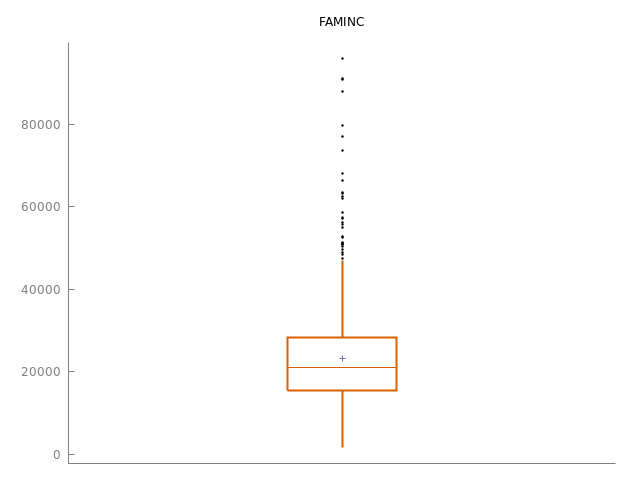
\includegraphics[width=1.0\textwidth]{../figures/boxplot.png}
				\caption{Boxplot}
			\end{figure}
	  \end{column}
	\end{columns}
\end{frame}


\begin{frame}[fragile]{Boxplot je Dummyausprägungen}
	\begin{columns}[T] % align columns
		\scriptsize
		\begin{column}{.55\textwidth}
			\begin{verbatim}
				set verbose off

				open mroz87.gdt

				boxplot FAMINC WE --factorized \
				  --output="boxplot_factorized.png" \
				  { set grid; set title "Foo" font ',15';\
				  set xlabel "Ausbildungsjahre" font ',14';}
			\end{verbatim}
		\end{column}

		\begin{column}{.47\textwidth}
			\begin{figure}
				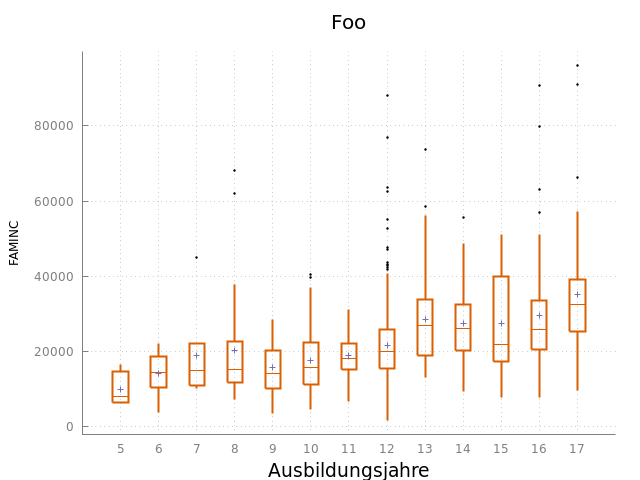
\includegraphics[width=1.0\textwidth]{../figures/boxplot_factorized.png}
				\caption{Boxplot je Ausbildungsjahr}
			\end{figure}
	  \end{column}
	\end{columns}
\end{frame}


\begin{frame}[fragile]{Kern-Dichte Plot}
	\begin{columns}[T] % align columns
		\scriptsize
		\begin{column}{.45\textwidth}
			\begin{verbatim}
				set verbose off

				open mroz87.gdt

				kdplot FAMINC --output=display
			\end{verbatim}
		\end{column}

		\begin{column}{.55\textwidth}
			\begin{figure}
				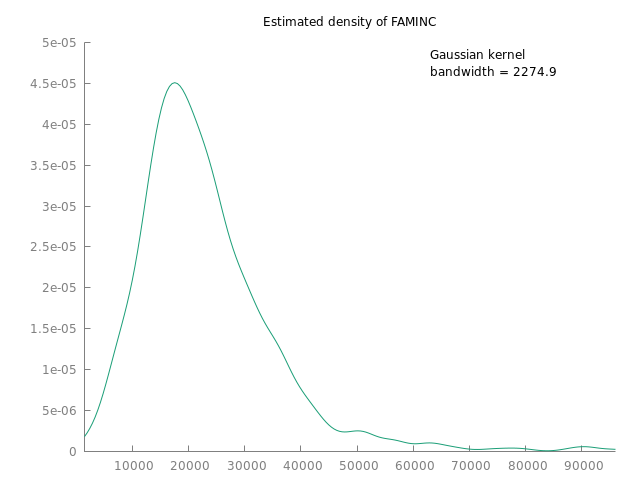
\includegraphics[width=1.0\textwidth]{../figures/kdplot.png}
				\caption{Kerndichteschätzung}
			\end{figure}
	  \end{column}
	\end{columns}
\end{frame}


\begin{frame}[fragile]{Histogramm}
	\begin{columns}[T] % align columns
		\scriptsize
		\begin{column}{.45\textwidth}
			\begin{verbatim}
				set verbose off

				open mroz87.gdt

				freq FAMINC --gamma --plot=display
			\end{verbatim}
		\end{column}

		\begin{column}{.55\textwidth}
			\begin{figure}
				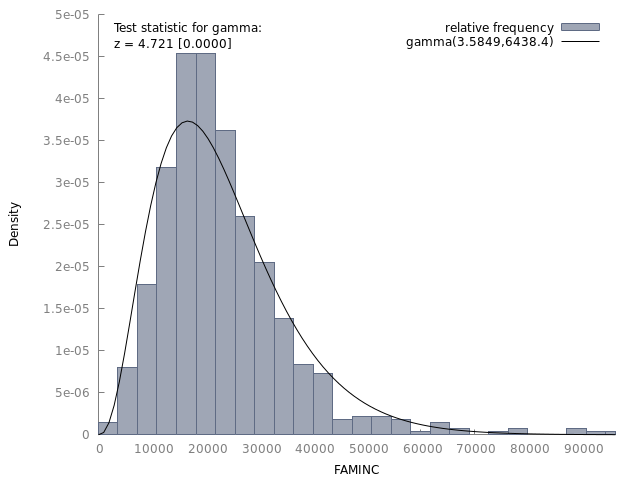
\includegraphics[width=1.0\textwidth]{../figures/freq_gamma.png}
				\caption{Histogramm mit Gamma-Verteilung}
			\end{figure}
	  \end{column}
	\end{columns}
\end{frame}


\begin{frame}[fragile]{Korrelationsmatrix}
	\begin{columns}[T] % align columns
		\scriptsize
		\begin{column}{.45\textwidth}
			\begin{verbatim}
				set verbose off

				open mroz87.gdt

				list L = 1..5
				corr L --triangle --plot=display
			\end{verbatim}
		\end{column}

		\begin{column}{.55\textwidth}
			\begin{figure}
				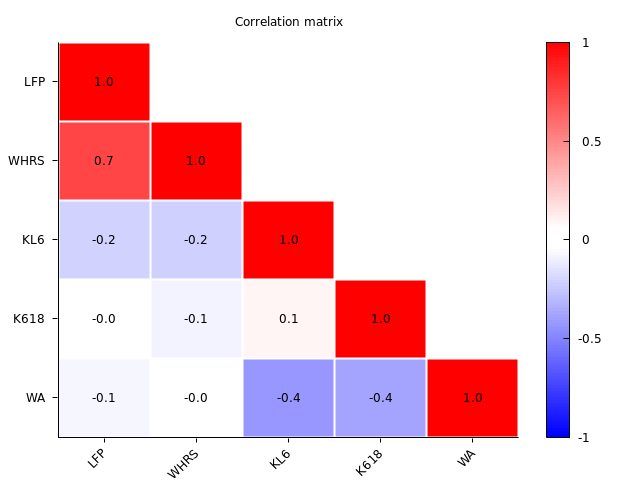
\includegraphics[width=1.0\textwidth]{../figures/correl_triangle.png}
				\caption{Korrelationsmatrix}
			\end{figure}
	  \end{column}
	\end{columns}
\end{frame}


\begin{frame}[fragile]{Gridplot}
	\begin{columns}[T] % align columns
		\scriptsize
		\begin{column}{.45\textwidth}
			\begin{verbatim}
				set verbose off
				open data4-10

				strings MyPlots

				gpbuild MyPlots
				  gnuplot ENROLL CATHOL
				  gnuplot ENROLL INCOME
				  gnuplot ENROLL COLLEGE
				  boxplot INCOME REGION --factorized
				end gpbuild

				gridplot MyPlots --output=display
			\end{verbatim}
		\end{column}

		\begin{column}{.55\textwidth}
			\begin{figure}
				\includegraphics[width=1.0\textwidth]{../figures/grdplot.png}
				\caption{Korrelationsmatrix}
			\end{figure}
	  \end{column}
	\end{columns}
\end{frame}


\begin{frame}[fragile]{Heatmap}
	\begin{columns}[T] % align columns
		\scriptsize
		\begin{column}{.5\textwidth}
			\begin{verbatim}
				open grunfeld.gdt --quiet
				# Install and load the package
				pkg install heatmap
				include heatmap.gfn
				# help heatmap

				# Restict sample to the first 4
				# panel units
				smpl $unit < 5 --restrict

				# Add information to the plot
				bundle Options = \
				  _(title = "Matrix A with contour lines",
				  quiet = TRUE, xlabel = "Time dimension",
				  ylabel = "Company")

				scalar T = $pd
				scalar N = $nobs / $pd
				matrix m = value

				matrix M = mshape(m, T, N)'
				heatmap(M, Options)

			\end{verbatim}
		\end{column}

		\begin{column}{.5\textwidth}
			\begin{figure}
				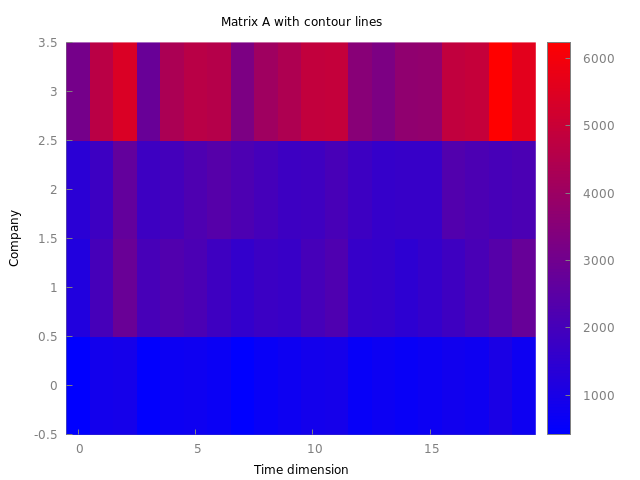
\includegraphics[width=0.8\textwidth]{../figures/heatmap.png}
				\caption{Heatmap}
			\end{figure}
	  \end{column}
	\end{columns}
\end{frame}


\begin{frame}[fragile]{Pair-Plots}
	\begin{columns}[T] % align columns
		\scriptsize
		\begin{column}{.5\textwidth}
			\begin{verbatim}
				pkg install PairPlot
				include PairPlot.gfn
				#help PairPlot

				open abdata --quiet
				list y = n k
				series factor = IND

				bundle opts = _(transparency_level = 175,
								  centroid = "median",
								  tics = FALSE,
								  pointsize = 1.5,
								  centroid_pointsize = 3,
								  centroid_linewidth = 3,
								  height = 600,
								  width = 600)

				PairPlot(y, factor, opts)
			\end{verbatim}
		\end{column}

		\begin{column}{.5\textwidth}
			\begin{figure}
				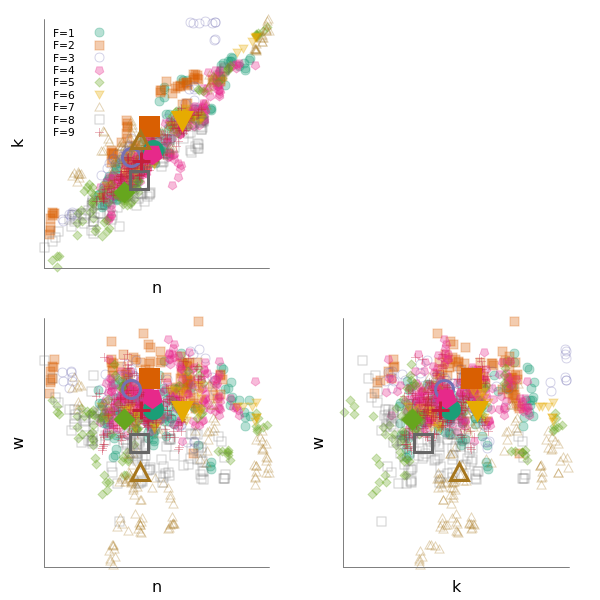
\includegraphics[width=0.9\textwidth]{../figures/pairplot_factorized.png}
				\caption{Kombinationen an Scatterplots mit Faktoren}
			\end{figure}
	  \end{column}
	\end{columns}
\end{frame}






%%%%%%%%%%%%%%%%%%%%%%%%%%%%%%%%%%%%
%%%%%%%%%%%%%%%%%%%%%%%%%%%%%%%%%%%%%%%%%%%%%%%%%%%%%%%%%%%%%%%%%%%%%%%%%
\section*{Referenzen}
\bibliographystyle{chicago}
\setcounter{secnumdepth}{0}

%\begin{frame}[allowframebreaks]
%	\frametitle{Literatur}
%	\footnotesize
%	\bibliography{../../../Dropbox/05_Literatur_DATENBANK/library}
%\end{frame}


%\section{Appendix}



\end{document}